\documentclass[../../main.tex]{subfiles}
% \documentclass[a4paper,10pt]{ltjsarticle}
\begin{document}
\rhead{京都大学後期$1997$年$3$番}
\setcounter{equation}{0}
\begin{oframed}
  \documentclass[../../main.tex]{subfiles}
\begin{document}

点$\mathrm{O}$を中心とする半径$1$の球面上に$4$点$\mathrm{A}$，$\mathrm{B}$，$\mathrm{C}$，$\mathrm{D}$があって
\begin{align*}
  \overrightarrow{\mathrm{OA}}+ \overrightarrow{\mathrm{OB}}+ \overrightarrow{\mathrm{OC}}+ \overrightarrow{\mathrm{OD}}=\vec{0}
\end{align*}
が成立しているとする．
\begin{enumerate}
  \item $|\overrightarrow{\mathrm{AB}}|=|\overrightarrow{\mathrm{CD}}|$であることを示せ．
  \item 点$\mathrm{B'}$，$\mathrm{D'}$を$\overrightarrow{\mathrm{OB'}}=-\overrightarrow{\mathrm{OB}}$，$\overrightarrow{\mathrm{OD'}}=-\overrightarrow{\mathrm{OD}}$となるようにとる．このとき$\mathrm{A}$，$\mathrm{B}'$，$\mathrm{C}$，$\mathrm{D}'$が互いに異なるならば，これら$4$点は，この順で，ある長方形の頂点となっていることを示せ．
\end{enumerate}

\end{document}

\end{oframed}
\setlength{\columnseprule}{0.4pt}
\begin{multicols}{2}
  {\bf [解答]}

  点 X の位置ベクトル (O 始点) を $\vec{x}$ と表すと，与式は
  \begin{align}
    \vec{a} + \vec{b} + \vec{c} + \vec{d} = 0 \label{eq:1}
  \end{align}
  である．また，各点が球面上にあるから
  \begin{align}
    |\vec{a}|=|\vec{b}|=|\vec{c}|=|\vec{d}|= 1 \label{eq:2}
  \end{align}
  である．

  \begin{figure}[H]
    \centering
    \tdplotsetmaincoords{70}{115} % 視点の角度を設定

    \begin{tikzpicture}[tdplot_main_coords, scale=1.8]
      % 球の輪郭は画面座標で円にする（xy 平面の円を投影すると楕円になる）．
      \begin{scope}[tdplot_screen_coords]
        \shade[ball color=blue!15!white, opacity=0.5] (0,0) circle (1);
        \draw[very thick, blue!85!black] (0,0) circle (1);
        \draw[densely dashed, gray!70!black] (-1,0) arc[start angle=180,end angle=360,x radius=1,y radius=0.28];
        \draw[gray!70!black] (1,0) arc[start angle=0,end angle=180,x radius=1,y radius=0.28];
      \end{scope}

      % 球の中心
      \coordinate (O) at (0,0,0);

      % 単位球面上かつ A+B+C+D=0 を満たす正四面体の頂点
      \pgfmathsetmacro{\invs}{1/sqrt(3)}
      \coordinate (A) at ({\invs}, {\invs}, {\invs});
      \coordinate (B) at ({\invs}, {-\invs}, {-\invs});
      \coordinate (C) at ({-\invs}, {\invs}, {-\invs});
      \coordinate (D) at ({-\invs}, {-\invs}, {\invs});

      % 正四面体の辺
      \draw[densely dashed, gray!70!black] (B) -- (C);
      \draw[thick, blue!85!black] (A) -- (B);
      \draw[thick, blue!85!black] (A) -- (C);
      \draw[thick, blue!85!black] (A) -- (D);
      \draw[thick, blue!85!black] (B) -- (D);
      \draw[thick, blue!85!black] (C) -- (D);

      % 点を描画
      \node[circle, fill=red!85!black, inner sep=1.4pt] at (A) {};
      \node[above=2pt, font=\small] at (A) {$A$};
      \node[circle, fill=red!85!black, inner sep=1.4pt] at (B) {};
      \node[below right=1pt, font=\small] at (B) {$B$};
      \node[circle, fill=red!85!black, inner sep=1.4pt] at (C) {};
      \node[above left=1pt, font=\small] at (C) {$C$};
      \node[circle, fill=red!85!black, inner sep=1.4pt] at (D) {};
      \node[below left=1pt, font=\small] at (D) {$D$};
    \end{tikzpicture}
    \caption{球面上に点$A,B,C,D$が配置されている様子（$\vec{a}+\vec{b}+\vec{c}+\vec{d}=\vec{0}$）}
    \label{1997-3:fig:1}
  \end{figure}

  \paragraph{(1)}
  \cref{eq:1}から
  \begin{align}
    \vec{a} + \vec{b} = -(\vec{c} + \vec{d})
  \end{align}
  だから，両辺2乗して, \cref{eq:2}を用いて
  \begin{align}
    \vec{a} \cdot \vec{b} = \vec{c} \cdot \vec{d} \label{eq:3}
  \end{align}
  となる．

  ここで，
  \begin{align}
    |\vec{a} - \vec{b}|^2
    & = |\vec{a}|^2 - 2\vec{a} \cdot \vec{b} + |\vec{b}|^2 \\
    & = 2 - 2\vec{a} \cdot \vec{b}                         \\
    |\vec{c} - \vec{d}|^2
    & =|\vec{c}|^2 - 2\vec{c} \cdot \vec{d} + |\vec{d}|^2  \\
    & = 2 - 2\vec{c} \cdot \vec{d}
  \end{align}
  だから，\cref{eq:3}よりこれらは等しく，
  \begin{align}
    & |\vec{a} - \vec{b}|^2 = |\vec{c} - \vec{d}|^2               \\
    \therefore
    & |\vec{a} - \vec{b}| = |\vec{c} - \vec{d}|                   \\
    & |\overrightarrow{\text{AB}}| = |\overrightarrow{\text{CD}}|
  \end{align}
  となる．よって題意は示された．  $\cdots$(答)

  \vspace{10pt}
  （2）
  AB'CD'が長方形をなすことを示すには，
  対角線ACとB'D'の長さが等しく，またその中点で交わることを示せばよい．

  \begin{figure}[H]
    \centering
    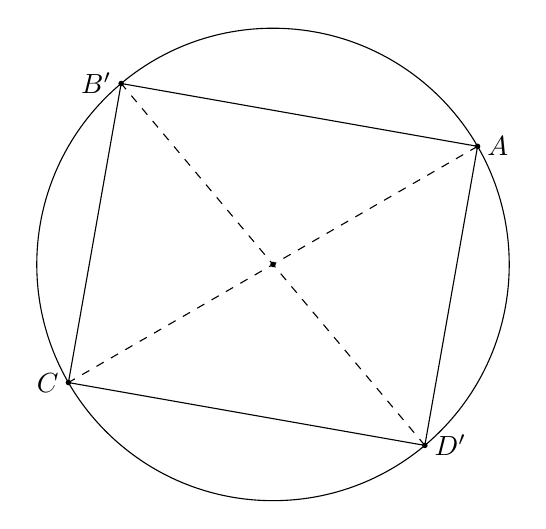
\begin{tikzpicture}[scale=3]
      \draw (0,0) circle (1);
      \coordinate (center) at (0,0);
      \coordinate (A) at ({cos(30)}, {sin(30)});
      \coordinate (B) at ({sin(40)}, {-cos(40)});
      \coordinate (B') at ({-sin(40)}, {cos(40)});
      \coordinate (C) at ({-cos(30)}, {-sin(30)});
      \coordinate (D) at ({-sin(40)}, {cos(40)});
      \coordinate (D') at ({sin(40)}, {-cos(40)});

      \draw (A) -- (B') -- (C) -- (D') -- cycle;

      \node at (center) [fill=black,inner sep=0pt,minimum size=2pt,circle] {};
      \node at (A) [fill=black,inner sep=0pt,minimum size=2pt,circle] {};
      \node at (B') [fill=black,inner sep=0pt,minimum size=2pt,circle] {};
      \node at (C) [fill=black,inner sep=0pt,minimum size=2pt,circle] {};
      \node at (D') [fill=black,inner sep=0pt,minimum size=2pt,circle] {};

      \node at (A) [right] {$A$};
      \node at (B') [left] {$B'$};
      \node at (C) [left] {$C$};
      \node at (D') [right] {$D'$};
      \draw[dashed] (A) -- (center) -- (C);
      \draw[dashed] (D') -- (center) -- (D);

    \end{tikzpicture}
    \caption{点A,B',C,D'の様子}
    \label{1997-3:fig:2}
  \end{figure}

  まずは対角線の長さACとB'D'を考える．
  題意より，$\vec{b}' = -\vec{b}, \vec{d}' = -\vec{d}$ である.
  \cref{eq:1}に代入して
  \begin{align}
    \vec{a} + \vec{c} = \vec{b}'+\vec{d}' \label{eq:4}
  \end{align}
  だから，
  (1) と同様に両辺二乗して\cref{eq:2}より
  \begin{align}
    \vec{a} \cdot \vec{c} = \vec{b}' \cdot \vec{d}'
  \end{align}
  であり，(1)と同様に
  \begin{align}
    |\overrightarrow{\text{AC}}| = |\overrightarrow{\text{B'D'}}|
  \end{align}
  となる．従って対角線の長さは等しい．

  次に，対角線ACとB'D'の交点がこれらの線分の中点であることを示す．
  \cref{eq:4}より
  \begin{align}
    \vec{p} = \dfrac{\vec{a} + \vec{c}}{2} = \dfrac{\vec{b}'+\vec{d}'}{2}
  \end{align}
  だから，ベクトル$\vec{p}$の表す点Pは線分AC，B'D'の中点である．
  従って点Pがこれらの交点かつ中点になっている．

  以上および，AB'CD'が互いに異なる点であることから，
  四角形 AB'CD' は長方形をなす．$\cdots$(答)

  \vspace{10pt}
  {\bf [解説]}

  % TODO :: これ，もっと強くA=-C, B=-Dが言えないのか？ -> 言えない

  % 又, AC と B'D' の交点の位置ベクトルを $\vec{x}$ は $t, s \in \mathbb{R}$ として
  % $t\vec{a} + (1-t)\vec{c} = -s\vec{b}' - (1-s)\vec{d}' = \vec{x}$
  % と表せる. $t=s=1/2$ はこの等式をみたし (ごちゃごちゃ). 2直線の
  % 交点はただ1つだから.
  % $\vec{x} = \dfrac{1}{2}(\vec{a} + \vec{c}) = \dfrac{1}{2}(\vec{b}' + \vec{d}')$

  % したがって.
  % $|\overrightarrow{\text{PA}}|^2 = \left|\dfrac{\vec{a}-\vec{c}}{2}\right|^2 = \left|-\dfrac{(\vec{a}-\vec{c})}{2}\right|^2 = |\overrightarrow{\text{PC}}|^2$
  % $|x| \ge 0$ から $|\overrightarrow{\text{PA}}| = |\overrightarrow{\text{PC}}|$ 同じく $|\overrightarrow{\text{PB}}| = |\overrightarrow{\text{PD}}|$ \quad $\cdots$ ③

  % ②, ③ と, A, B', C, D' が互いに異なる点であることから,

  \newpage
\end{multicols}
\end{document}
